% Insert at the Task 4 position; uses existing amsmath, graphicx, booktabs/longtable.
% Figure paths are relative to simple_assessment. This fragment defines no document class or packages.
\section{5. Scenario-Based Robustness and Sustainability
Assessment}\label{sec:task4-scenario-based-robustness-and-sustainability-assessment}

\subsection{5.1 Robustness Assessment
Framework}\label{sec:task4-robustness-assessment-framework}

SWITCH must assess whether routing benefits survive changes in workload
and prediction reliability. The assessment retains Task 2's frozen
Pre-LightGBM direct router with its finite-sample risk guard and Task
3's final Spatial MILP + DES. Four scenarios compare the baseline of
7,335 requests with a 40\% Math/Code share at unchanged volume,
prediction error, and approximately 50\% demand growth to 11,002
requests. Prediction error adds independent \(\mathcal N(0,0.10^2)\)
perturbations to the two saved quality predictions before clipping to
\([0,1]\), then reapplies the frozen routing rule; duplicates share
prompt-group perturbations. Math, Code and unregistered-source fallbacks
remain L.

Each scenario uses three paired Greedy/Spatial seeds with identical
routing, requests, six hosts and exogenous randomness: 24 executions
over \(H=43{,}200\) s. Scheduling retains its causal information
boundary; historical quality and future actual carbon are evaluation
data. Summaries average seed-level quantities, including ratios and
completed-request P95s. Three seeds support descriptive comparisons;
replayed requests add no independent quality observations.

For historical score \(q_{i,m_i}\) and Task 3's violation indicator
\(V_i\), define

\[
\begin{aligned}
Q&=\frac1N\sum_i q_{i,m_i},& P_{\mathrm{hist}}&=\frac1N\sum_i\mathbf1\{q_{i,m_i}\ge0.5\},\\
P_{\mathrm{valid}}&=\frac1N\sum_i(1-V_i)\mathbf1\{q_{i,m_i}\ge0.5\},&
\mathrm{Violation}&=\frac1N\sum_i V_i.
\end{aligned}
\tag{5.1}
\]

Failure, excessive waiting, late completion and window censoring count
as violations. Historical quality is distinct from compliant delivery;
completed-request P95 accompanies all-input service risk.

\subsection{5.2 Robustness Under Three Stress
Scenarios}\label{sec:task4-robustness-under-three-stress-scenarios}

\textbf{Higher Share of Math/Code Requests.} Increasing their share
raises Spatial's P95 from 7.827 to 11.967 s, while violations remain
0.0182\%. Mean historical Score falls from 0.776142 to 0.748728, but
historical pass rate rises from 83.817\% to 84.872\%. This is consistent
with the baseline Math distribution: its mean Score is lower than
General's (0.6624 versus 0.8125), but its threshold-pass rate is higher
(91.99\% versus 81.51\%). Mean score and threshold probability need not
move together. The scenario represents task composition and
computational load, rather than greater intrinsic difficulty for every
request.

\textbf{Prediction Error.} Per seed, 133-139 requests change model
choice: L-to-S counts are 67/75/68 and S-to-L counts are 70/64/65, all
in General. Comparing the same changed requests using their paired
historical S/L scores identifies 19/22/18 declines of at least 0.10
Score, a descriptive reporting threshold. Among new S choices, 13/15/12
lose an answer that L would have passed. The small population-average
change conceals these local harms: fewer than 2\% of requests switch,
approximately 71.63\% of switches have identical S/L scores, and gains
offset losses. The fallback prevents Math/Code switches here; no
guard-removal ablation or renewed statistical coverage under noise is
established.

\textbf{Demand Growth.} At 11,002 requests, Spatial's violations rise
from 0.0182\% to 0.1697\% and P95 to 11.885 s; completion is 99.8303\%.
Growth Greedy has more violations (1.6270\%) but lower completed-request
P95 (6.998 s). Spatial therefore trades longer observed tail response
for fewer violations. Different completed sets preclude interpreting P95
alone as overall service superiority.



\subsection{5.3 Carbon Rebound and Total Environmental
Impact}\label{sec:task4-carbon-rebound-and-total-environmental-impact}

The unchanged facility boundary is

\[
C_{\mathrm{total}}=C_{\mathrm{idle}}+C_{\mathrm{active}}+C_{\mathrm{net}}+C_{\mathrm{ctrl}},
\qquad C_{\mathrm{op}}=C_{\mathrm{total}}-C_{\mathrm{idle}}.
\tag{5.2}
\]

The active term accounts for electricity above idle; network and
controller costs remain separate. All powered hosts retain their
full-window idle charge. Baseline Greedy emits 41,288.178 gCO2e and
Spatial 41,214.556 gCO2e: a same-demand saving of 73.622 gCO2e, or
0.1783\%. Fixed idle contributes 41,140.3512 gCO2e, approximately
99.82\% of baseline Spatial's total. This is an accounting share, not
idle-time utilization or a removable energy budget. Spatial uses
approximately 0.004857 kWh more electricity while emitting less carbon:
carbon efficiency is not necessarily equivalent to energy efficiency.

\begin{center}
\begin{minipage}{\linewidth}
\centering
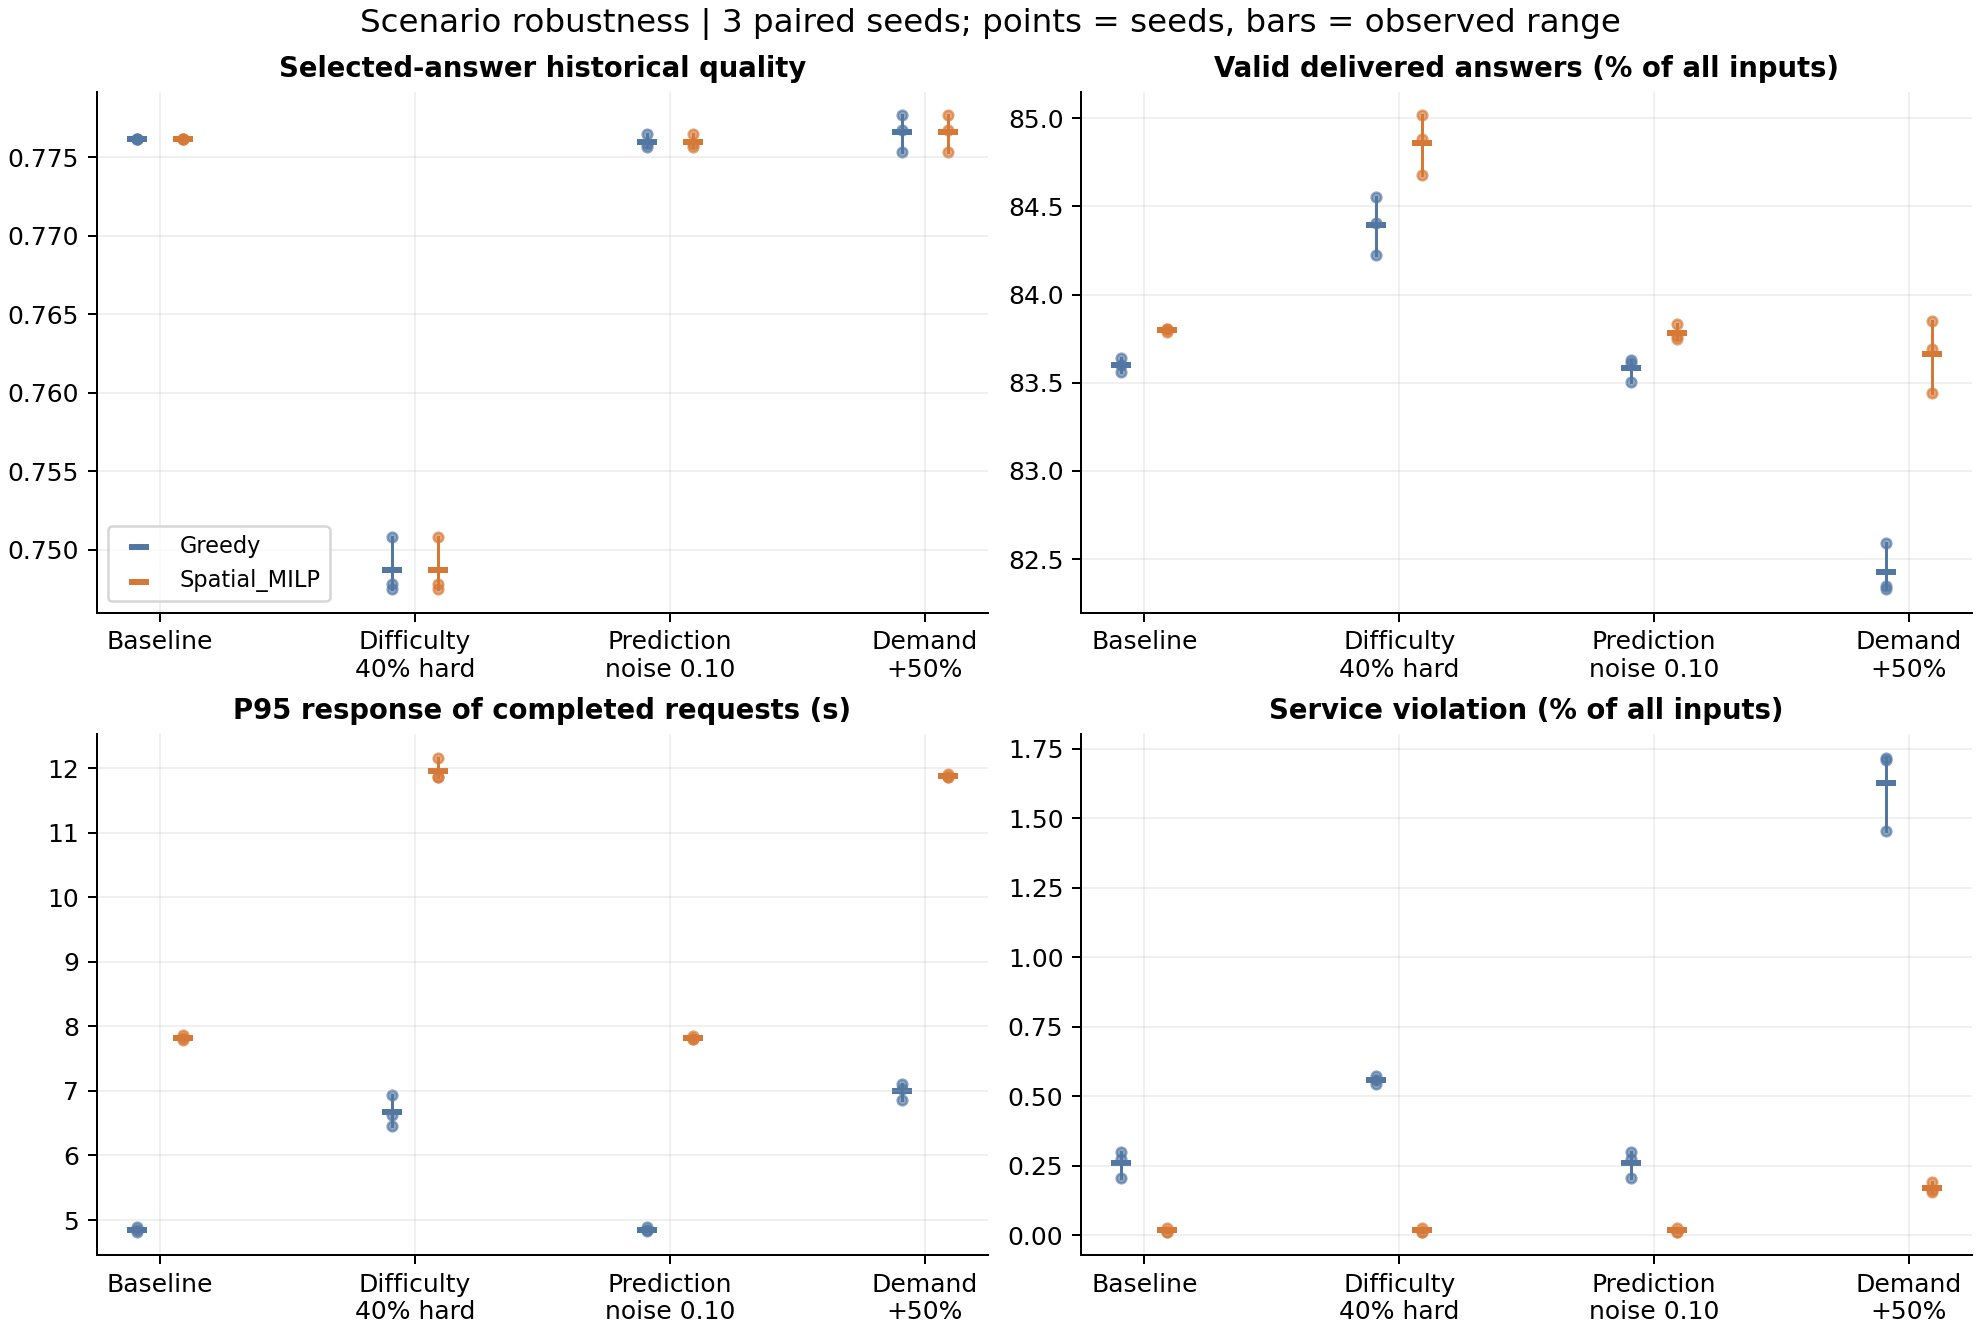
\includegraphics[width=0.90\linewidth]{figures/Figure1_Robustness.png}
\captionof{figure}{Paired scenario results. Points denote seeds, horizontal
marks means, and vertical bars observed ranges. P95 is conditional on
completion; violation and valid-pass rates use all inputs. The original
label ``Difficulty 40\% hard'' means a 40\% Math/Code share.}
\label{fig:task4-robustness}
\end{minipage}
\end{center}

Let \(C_G(N)\) and \(C_{\mathrm{Sp}}(N)\) denote total carbon under
Greedy and Spatial at demand \(N\). With \(N_0=7{,}335\) and
\(N_1=11{,}002\), the paired mean contrasts are

\[
\begin{aligned}
C_G(N_1)-C_{\mathrm{Sp}}(N_1)&=101.443\ \mathrm{gCO2e},\\
C_{\mathrm{Sp}}(N_1)-C_G(N_0)&=+2.496\ \mathrm{gCO2e}.
\end{aligned}
\tag{5.3}
\]

Spatial still saves carbon at matched increased demand, yet its growth
total, 41,290.674 gCO2e, exceeds original-demand Greedy by approximately
0.006045\%. These comparisons answer different questions. The small
reversal is conditional on power, PUE and carbon-intensity assumptions;
its real-world sign and magnitude are unverified.

Growth also changes where computation occurs. France's share of
Spatial's active electricity falls from 89.583\% to 79.632\%, while
execution-weighted active carbon intensity rises from 42.237 to 57.231
gCO2e/kWh. The regional hourly carbon series are unchanged: execution
weights shift toward more carbon-intensive regions. Consequently the
baseline per-input operational carbon coefficient is not constant under
growth.

Under fixed idle and constant
\(c_0=[C_{\mathrm{Sp}}(N_0)-C_{\mathrm{idle}}]/N_0>0\), the linear
reference \(C_{\mathrm{Sp}}^{\mathrm{lin}}(N)=C_{\mathrm{idle}}+Nc_0\)
yields

\[
r_{\mathrm{lin}}=\frac{C_G(N_0)-C_{\mathrm{Sp}}(N_0)}{C_{\mathrm{Sp}}(N_0)-C_{\mathrm{idle}}}.
\tag{5.4}
\]

Its seed-mean value, 99.21\%, is algebraically correct under those
assumptions, but is not a DES rebound threshold. Only zero and
approximately 50\% growth were simulated; an accurate nonlinear crossing
is unidentified. Moreover, growth was imposed externally. Without
demand-elasticity evidence, this comparison cannot establish that
efficiency improvements caused increased use.

\begin{center}
\begin{minipage}{\linewidth}
\centering
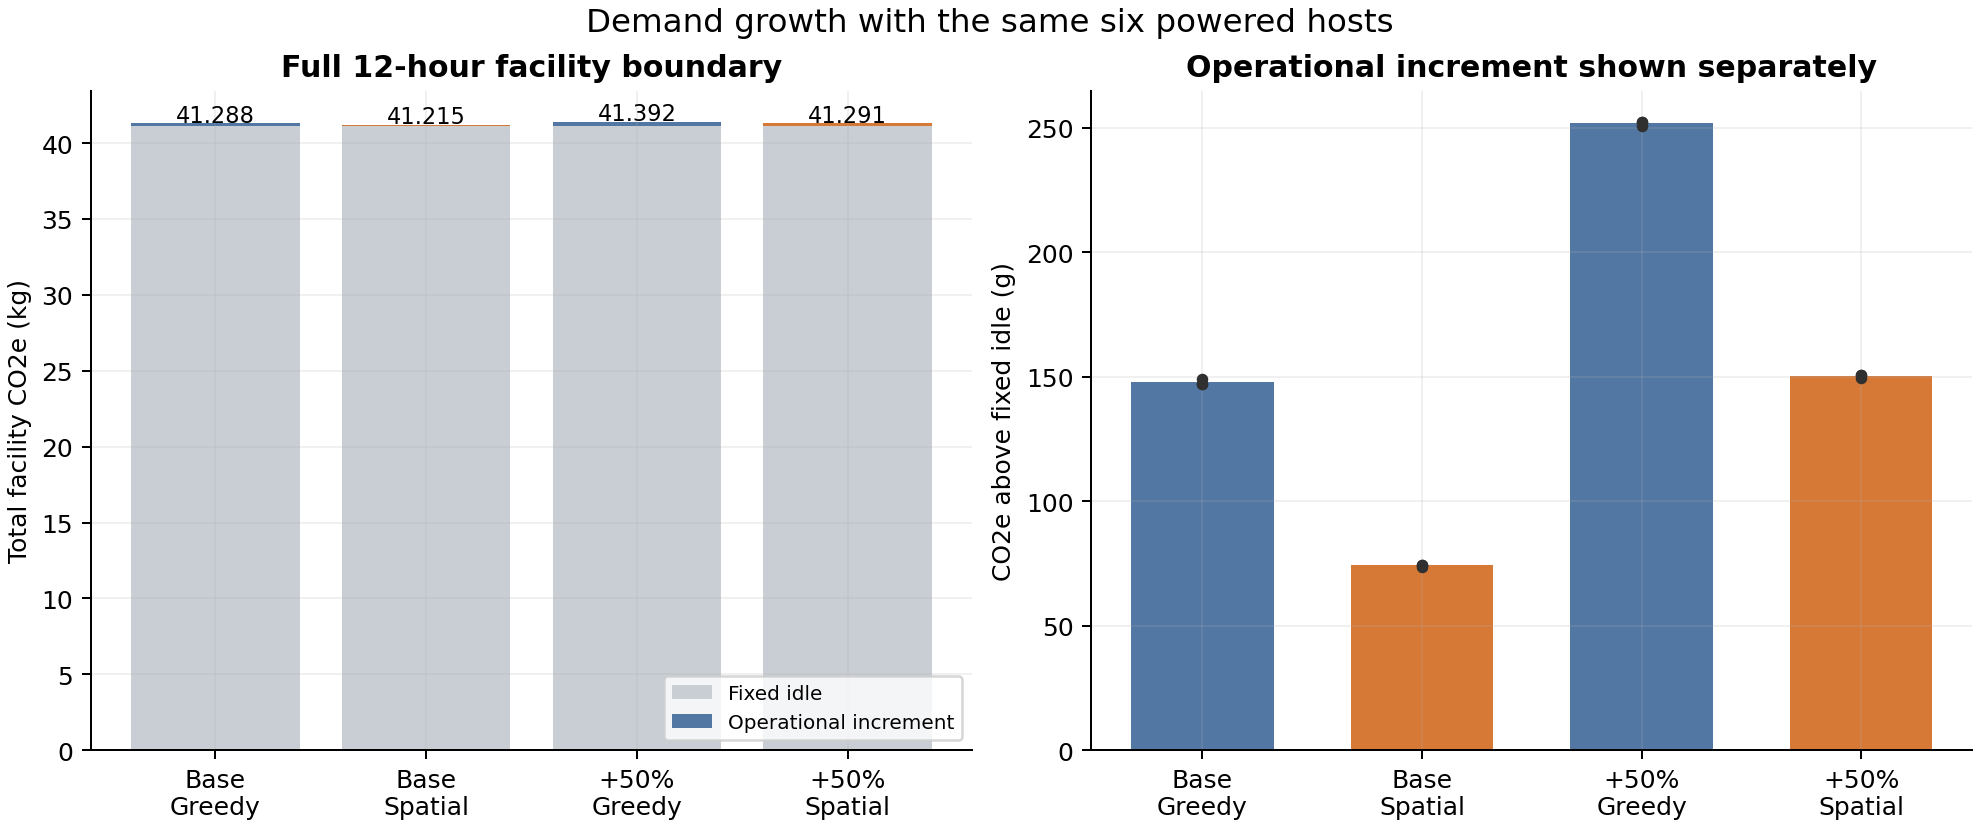
\includegraphics[width=\linewidth]{figures/Figure2_Carbon_Growth.png}
\captionof{figure}{The left panel includes fixed idle and uses kgCO2e; the
right isolates operational increments in gCO2e. Greedy versus Spatial
within demand measures scheduling savings; growth Spatial versus
baseline Greedy measures the cross-demand total change.}
\label{fig:task4-carbon}
\end{minipage}
\end{center}

\subsection{5.4 Fairness Across Request
Types}\label{sec:task4-fairness-across-request-types}

Routing quality and scheduling service require separate comparisons.
Using paired historical scores, the routing contrast is
\(\Delta Q_g=N_g^{-1}\sum_{i\in g}(q_{i,m_i}-q_{i,L})\). Baseline
General has Router/All-L means 0.812466/0.818424, a difference of
-0.005958 and a pass-rate difference of -0.5055 percentage points.
Math/Code choose L throughout, giving zero reference differences, rather
than perfect absolute quality. L does not dominate S on every request.
All-L is solely an offline quality reference, with no simulated All-L
service or carbon counterfactual.

Across the 36 task-by-scenario-by-seed comparisons, Spatial never
increases observed category violations relative to Greedy, but
completed-request P95 is generally higher. Table~\ref{tab:task4-growth} shows growth
outcomes. Code has the highest Spatial violation rate and largest
increase from baseline, yet its 86 baseline instances contain only 85
distinct prompt groups; duplication adds no independent quality
evidence. Task comparisons neither establish demographic fairness nor
exclude other systematic harms.

\refstepcounter{table}\label{tab:task4-growth}\emph{Table \thetable. Growth scenario, seed means. Each cell is Greedy/Spatial.
Rates use all inputs; P95 uses completions. Valid pass requires both
historical quality and compliant delivery.}

{\def\LTcaptype{none} % do not increment counter
\begingroup
\AtBeginEnvironment{longtable}{\footnotesize}
\begin{longtable}[]{@{}
  >{\raggedright\arraybackslash}p{(\linewidth - 8\tabcolsep) * \real{0.2000}}
  >{\raggedright\arraybackslash}p{(\linewidth - 8\tabcolsep) * \real{0.2000}}
  >{\raggedright\arraybackslash}p{(\linewidth - 8\tabcolsep) * \real{0.2000}}
  >{\raggedright\arraybackslash}p{(\linewidth - 8\tabcolsep) * \real{0.2000}}
  >{\raggedright\arraybackslash}p{(\linewidth - 8\tabcolsep) * \real{0.2000}}@{}}
\toprule\noalign{}
\begin{minipage}[b]{\linewidth}\raggedright
Task
\end{minipage} & \begin{minipage}[b]{\linewidth}\raggedright
Violation (\%)
\end{minipage} & \begin{minipage}[b]{\linewidth}\raggedright
Completion (\%)
\end{minipage} & \begin{minipage}[b]{\linewidth}\raggedright
P95 (s)
\end{minipage} & \begin{minipage}[b]{\linewidth}\raggedright
Valid pass (\%)
\end{minipage} \\
\midrule\noalign{}
\endhead
\bottomrule\noalign{}
\endlastfoot
General & 1.5925/0.1404 & 98.408/99.860 & 4.896/10.502 &
80.247/81.438 \\
Math & 1.7354/0.2482 & 98.265/99.752 & 8.493/13.945 & 90.293/91.703 \\
Code & 1.7590/0.4919 & 98.241/99.508 & 12.211/18.329 & 67.435/68.204 \\
\end{longtable}
\endgroup
}

\subsection{5.5 Environmental Evidence and
Limitations}\label{sec:task4-environmental-evidence-and-limitations}

Table~\ref{tab:task4-evidence} separates environmental observations, transferred parameters and
assumptions from deployment evidence still needed.

\refstepcounter{table}\label{tab:task4-evidence}\emph{Table \thetable. Evidence supporting the assessment and its limits.}

{\def\LTcaptype{none} % do not increment counter
\begingroup
\AtBeginEnvironment{longtable}{\footnotesize}
\begin{longtable}[]{@{}
  >{\raggedright\arraybackslash}p{(\linewidth - 2\tabcolsep) * \real{0.5000}}
  >{\raggedright\arraybackslash}p{(\linewidth - 2\tabcolsep) * \real{0.5000}}@{}}
\toprule\noalign{}
\begin{minipage}[b]{\linewidth}\raggedright
Evidence used
\end{minipage} & \begin{minipage}[b]{\linewidth}\raggedright
What remains unestablished
\end{minipage} \\
\midrule\noalign{}
\endhead
\bottomrule\noalign{}
\endlastfoot
RouterBench paired historical S/L scores & Representative public-sector
quality and demand \\
Historical hourly DE/FR/ES carbon intensity & Original forecast vintages
and marginal-grid effects \\
GPU power proxy transferred from published measurements & Actual power
of the target models on their serving hardware \\
Assumed idle power, PUE, arrivals and service times & Site telemetry,
calibrated queues and facility PUE \\
Conditional DES execution and complete energy ledger & Measured
deployment savings and a suitable causal counterfactual \\
\end{longtable}
\endgroup
}

Historical average intensity supports attributional accounting, not
marginal-grid causality. SWITCH should require measured site energy and
PUE, representative quality and service audits, and monitoring of demand
and task-level harms. Matched-demand carbon savings here assure neither
lower electricity consumption, shorter responses, nor lower totals after
growth.
